\chapter{The Degrees-of-Freedom Problem}
\label{ch:dof-problem}

\epigraph{%
  The coordination of movement is the process of mastering redundant
  degrees of freedom of the moving organ, in other words its conversion
  to a controllable system.
}{--- Nikolai Bernstein, 1967}

\section{Bernstein's Original Formulation}

In 1935, Nikolai Bernstein, a Soviet physiologist, made a deceptively simple
observation: the number of degrees of freedom available for any motor task
\emph{vastly exceeds} the number required to define the task. This observation,
formalized in his 1967 monograph \cite{Bernstein1967}, is the founding problem
of motor control.

\begin{definition}{The Degrees-of-Freedom Problem}{dof-problem}
  Let a motor task be defined by $k$ task-space constraints (e.g., $k = 6$ for
  placing a hand at a specific position and orientation). Let the body have $n$
  joint degrees of freedom and $p > n$ muscles. The \textbf{degrees-of-freedom
  problem} is: how does the nervous system select a specific solution
  $(\bm{q}(t), \bm{u}(t)) \in \Reals^n \times \Reals^p$ from the infinite set
  of solutions consistent with the task constraints?

  The \textbf{kinematic redundancy} is $n - k$ (extra joint configurations).
  The \textbf{muscle redundancy} is $p - n$ (extra muscles per joint).
  The \textbf{total redundancy} is $(n - k) + (p - n) = p - k$.
\end{definition}

\subsection{The Numbers Are Staggering}

Consider the golf swing:
\begin{center}
\renewcommand{\arraystretch}{1.3}
\begin{tabular}{@{}lr@{}}
\toprule
\textbf{Quantity} & \textbf{Approximate Value} \\
\midrule
Skeletal DOF involved & $\sim$200 \\
Muscles contributing & $\sim$400 \\
Task constraints (clubhead at impact) & 6 \\
Kinematic redundancy & $\sim$194 \\
Muscle redundancy & $\sim$200 \\
Total redundancy & $\sim$394 \\
Duration of downswing & $\sim$0.25~s \\
Neural processing delay & $\sim$0.1$\,$--$\,$0.2~s \\
\bottomrule
\end{tabular}
\end{center}

The nervous system must select from $\sim$400-dimensional muscle activation patterns
to satisfy 6 constraints, while accounting for interaction torques, gravity, and
neural delays---\emph{in a quarter of a second}. This is the problem.

\begin{figure}[h]
\centering
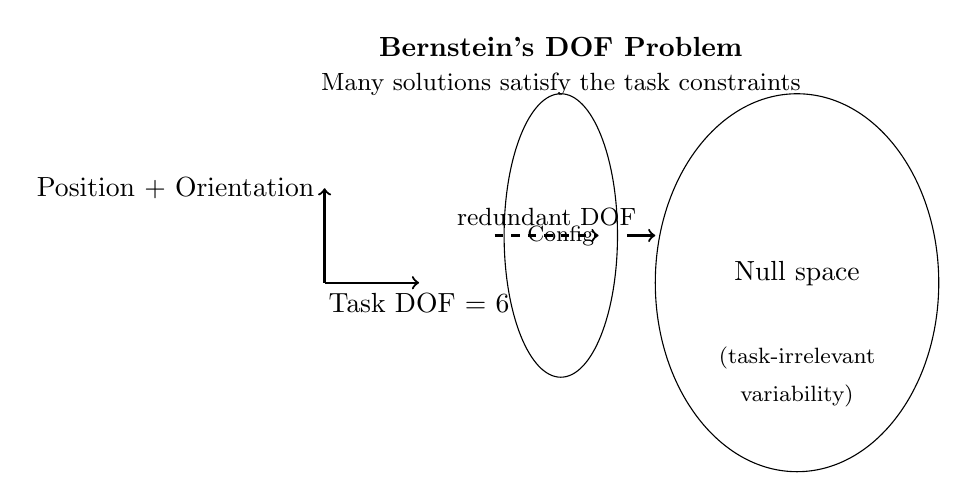
\begin{tikzpicture}[scale=1.2]
  % Task space (low-dim)
  \draw[->, thick] (0, 0) -- (1, 0) node[align=center, anchor=north] {Task DOF = 6};
  \draw[->, thick] (0, 0) -- (0, 1) node[align=center, anchor=east] {Position + Orientation};

  % Mapping to configuration space
  \draw (2.5, 0.5) ellipse (0.6 and 1.5) node[align=center, anchor=center] {\footnotesize Config};

  % Null space visualization
  \draw (5, 0) ellipse (1.5 and 2);
  \draw (5, 0.1) node[align=center, anchor=center] {Null space};
  \draw (5, -0.8) node[align=center, anchor=center] {\footnotesize (task-irrelevant};
  \draw (5, -1.2) node[align=center, anchor=center] {\footnotesize variability)};

  % Arrow showing redundancy
  \draw[->, thick, dashed] (1.8, 0.5) -- (2.9, 0.5) node[align=center, anchor=south, midway] {\small redundant DOF};
  \draw[->, thick] (3.2, 0.5) -- (3.5, 0.5);

  % Label
  \draw (2.5, 2.5) node[align=center, anchor=center] {\textbf{Bernstein's DOF Problem}};
  \draw (2.5, 2.1) node[align=center, anchor=center] {\small Many solutions satisfy the task constraints};
\end{tikzpicture}
\caption{The degrees-of-freedom problem: redundancy in configuration space allows
task-irrelevant variability in the null space of the task Jacobian.}
\label{fig:ch1:dof-illustration}
\end{figure}

\section{From Problem to Resource: Motor Abundance}

Modern motor control theory has reframed Bernstein's ``problem'' as an
\emph{opportunity}. Redundancy is not a curse but a resource:

\begin{insight}{Redundancy as Motor Abundance}{abundance}
  The extra degrees of freedom provide:
  \begin{enumerate}
    \item \textbf{Flexibility}: the same task can be performed in many ways,
          allowing adaptation to constraints (fatigue, injury, obstacles)
    \item \textbf{Robustness}: perturbations can be absorbed without task failure
    \item \textbf{Exploration}: variability in execution allows the system to
          discover better solutions over time
    \item \textbf{Error correction}: task-irrelevant DOF can compensate for
          errors in task-relevant DOF
  \end{enumerate}
  We adopt the term \textbf{motor abundance} (Latash 2012) to emphasize that
  redundancy is a feature, not a bug.
\end{insight}

\section{The Uncontrolled Manifold Hypothesis}

The uncontrolled manifold (UCM) hypothesis \cite{ScholzSchoner1999} provides a
mathematical framework for understanding how the nervous system manages redundancy.

\begin{definition}{The Uncontrolled Manifold}{ucm}
  Let $\bm{q} \in \Reals^n$ be the joint configuration and $\bm{y} = h(\bm{q}) \in \Reals^k$
  be the task variable. The \textbf{uncontrolled manifold} at a nominal configuration
  $\bm{q}_0$ is the null space of the task Jacobian:
  \begin{equation}
    \text{UCM}(\bm{q}_0) = \left\{ \delta\bm{q} \in \Reals^n :
    J_h(\bm{q}_0) \delta\bm{q} = \bm{0} \right\},
    \label{eq:ch1:ucm-def}
  \end{equation}
  where $J_h = \partial h / \partial \bm{q}$ is the task Jacobian. Variability within
  the UCM does not affect the task variable. Variability perpendicular to the UCM
  (in the \textbf{orthogonal complement}) directly affects task performance.
\end{definition}

\begin{laymansbox}{Mathematical Reminder: The Geometry of the UCM}{ucm_geometry_reminder}
Recall our differential geometry from Volume 0: a manifold is a curved surface representing valid states. The \textbf{Uncontrolled Manifold} (UCM) is quite literally a geometric submanifold embedded inside the larger configuration space $\mathcal{Q}$. 

Because the task geometry is non-linear (e.g., the arc of a swinging robot arm), the UCM is curved. We calculate its flat \textbf{Tangent Space} mathematically using the null space of the Jacobian ($J_h \delta\bm{q} = \bm{0}$). As long as the nervous system's noise vectors point exclusively into this tangent space, the physical position of the hand will not budge from the target. The nervous system is actively shaping its noise ellipsoid to align with the tangent space of the target manifold!
\end{laymansbox}

The UCM hypothesis predicts that the nervous system:
\begin{enumerate}
  \item \textbf{Suppresses} variability in the orthogonal complement of the UCM
        (task-relevant variability)
  \item \textbf{Tolerates} or even \textbf{encourages} variability within the UCM
        (task-irrelevant variability)
\end{enumerate}

This has been experimentally confirmed across many motor tasks \cite{ScholzSchoner1999,
Todorov2002}.

\begin{lstlisting}[language=Python, caption={Uncontrolled manifold analysis.}]
import numpy as np
from typing import Tuple

def ucm_analysis(
    joint_angles: np.ndarray,
    task_jacobian_func,
    n_repetitions: int | None = None
) -> Tuple[float, float, float]:
    """Perform UCM variance decomposition.

    Parameters
    ----------
    joint_angles : np.ndarray, shape (n_reps, n_dof)
        Joint angle data from multiple repetitions of the same task.
    task_jacobian_func : callable
        q -> J(q), shape (k, n_dof), the task Jacobian.
    n_repetitions : int, optional
        Number of repetitions (inferred from data if not given).

    Returns
    -------
    Tuple[float, float, float]
        (variance_ucm, variance_ort, ratio)
        UCM variance, orthogonal variance, and their ratio.
    """
    n_reps, n_dof = joint_angles.shape
    q_mean = np.mean(joint_angles, axis=0)

    # Task Jacobian at the mean configuration
    J = task_jacobian_func(q_mean)
    k = J.shape[0]  # task dimension

    # Null space of J (UCM directions)
    U, S, Vt = np.linalg.svd(J, full_matrices=True)
    rank = np.sum(S > 1e-10)
    null_space = Vt[rank:].T  # Shape: (n_dof, n_dof - rank)

    # Orthogonal complement (range space)
    range_space = Vt[:rank].T  # Shape: (n_dof, rank)

    # Decompose variability
    deviations = joint_angles - q_mean  # (n_reps, n_dof)

    # Project onto UCM
    proj_ucm = deviations @ null_space  # (n_reps, n_dof - rank)
    var_ucm = np.mean(np.sum(proj_ucm**2, axis=1))

    # Project onto orthogonal complement
    proj_ort = deviations @ range_space  # (n_reps, rank)
    var_ort = np.mean(np.sum(proj_ort**2, axis=1))

    # Normalize by dimensionality
    var_ucm_per_dof = var_ucm / (n_dof - rank) if n_dof > rank else 0
    var_ort_per_dof = var_ort / rank if rank > 0 else 0

    ratio = var_ucm_per_dof / var_ort_per_dof if var_ort_per_dof > 0 else np.inf

    return var_ucm_per_dof, var_ort_per_dof, ratio


# Example: 3-joint planar arm reaching to a point
def planar_arm_jacobian(q: np.ndarray, L: np.ndarray = np.array([0.3, 0.25, 0.2])):
    """Task Jacobian for endpoint position of a 3-link planar arm."""
    n = len(q)
    J = np.zeros((2, n))
    for i in range(n):
        for j in range(i, n):
            angle_sum = np.sum(q[:j+1])
            J[0, i] -= L[j] * np.sin(angle_sum)
            J[1, i] += L[j] * np.cos(angle_sum)
    return J

# Generate synthetic reaching data (50 repetitions)
np.random.seed(42)
q_nominal = np.array([0.5, 1.2, -0.3])
n_reps = 50
# Motor noise: more variability in task-irrelevant directions
noise = np.random.randn(n_reps, 3) * 0.05
q_data = q_nominal + noise

v_ucm, v_ort, ratio = ucm_analysis(q_data, planar_arm_jacobian)
print(f"UCM variance (per DOF): {v_ucm:.6f}")
print(f"ORT variance (per DOF): {v_ort:.6f}")
print(f"UCM/ORT ratio:          {ratio:.2f}")
print(f"(Ratio > 1 supports the UCM hypothesis)")
\end{lstlisting}

\section{Bernstein's Three Stages of Learning}

Bernstein proposed that motor skill acquisition progresses through three stages:

\begin{enumerate}
  \item \textbf{Freezing}: initially, the learner constrains (``freezes'') excess
        degrees of freedom, reducing the system to manageable dimensionality.
        A beginner golfer keeps wrists rigid, eliminating the wrist DOF.
  \item \textbf{Freeing}: as skill develops, the learner gradually releases
        (``frees'') the frozen DOF, allowing them to participate in the movement.
        The intermediate golfer adds wrist hinge.
  \item \textbf{Exploiting}: the expert learner exploits the released DOF to
        harness reactive forces, elastic energy, and passive dynamics. The expert
        golfer uses the passive wrist release driven by centrifugal force.
\end{enumerate}

In the language of control theory:
\begin{itemize}
  \item Stage 1: reduce the system dimension from $n$ to $k$ (the task dimension)
  \item Stage 2: increase the controlled dimension while maintaining task performance
  \item Stage 3: exploit the drift dynamics $f(\state)$ by designing trajectories that
        use passive mechanics (Volume~II, Chapter~5)
\end{itemize}

\section*{Exercises}

\begin{enumerate}
  \item \textbf{Redundancy Quantification.}
        For each of the following tasks, estimate the task dimension $k$, body DOF $n$,
        and compute the kinematic redundancy:
        (a) Standing balance, (b) Picking up a cup, (c) Walking on a treadmill,
        (d) A tennis serve.

  \item \textbf{UCM Analysis.}
        Using the provided code, generate synthetic data for 3-joint planar reaching
        with structured variability (more noise in the null space of the Jacobian).
        Verify that the UCM/ORT ratio exceeds 1.

  \item \textbf{Bernstein's Stages.}
        Observe a beginner and an expert performing the same motor task (e.g., throwing
        a ball). Describe their movement in terms of Bernstein's three stages. Which
        degrees of freedom are frozen, freed, and exploited?

  \item \textbf{(Programming.)} Implement a UCM analysis for a 7-DOF arm model reaching
        to a 3D target. Visualize the UCM and ORT directions.

  \item \textbf{(Research.)} Read Scholz and Sch{\"o}ner (1999) and summarize the key
        experimental evidence for the UCM hypothesis.
\end{enumerate}
